\subsection{Related Standards}
\begin{flushleft}
    % C++
    C++ will be programmed according to the C++20 standard, formally known as
    \href{https://www.iso.org/standard/79358.html}{ISO/IEC 14882:2020}. C++ is
    a superset of C, and builds upon it by introducing object-oriented
    programming concepts while maintaining the functional language aspect of C.
\end{flushleft}
\begin{flushleft}
    % 802.11
    The microcontroller (MCU) supports transmission through the Institute of
    Electrical and Electronics Engineers (IEEE) 802.11b/g/n standard of wireless
    communication. This standard uses the S band of radio frequences and
    operates at 2.4 GHz. There are 14 accessible channels, each spanning a band
    width of 22 MHz (pictured in\autoref{wifi_channels}).
    \begin{figure}[H]
        \caption{802.11b/g/n channels}
        \label{wifi_channels}
        \centering
        
\includegraphics[width=0.75\textwidth]{images/wifi_channels.png}
    \end{figure}
    These channels specifically reside in an industrial, scientific and medical
    (ISM) band. This standard also provides datagram frames for the transport
    layer.
\end{flushleft}
\begin{flushleft}
    % TCP
    Transmission Control Protocol (TCP) will be used to satisfy transport layer
    requirements of the product, and will be used to transmit symbols (i.e.
    from any commands, data, settings, telemetry, etc.) between Amazon Web
    Services (AWS) and the microcontroller (MCU). TCP was chosen over other
    protocols, such as User Datagram Protocol (UDP), mainly due to its
    reliability. The extent of TCP's reliability includes features such as
    checksums, duplicate data detection, retrying of transmissions, sequencing,
    and timers.
    Such reliability is favored over higher bandwidth or lower
    latency, as neither of the latter are required for the kilobytes
    of information being relayed between AWS and the MCU. A standard TCP frame
    is shown in \autoref{tcp_frame}.
    \begin{figure}[H]
        \caption{TCP frame (\href{https://condor.depaul.edu/jkristof/technotes/tcp.html}{The Transmission Control Protocol}, Fig. 1)}
        \label{tcp_frame}
        \centering
        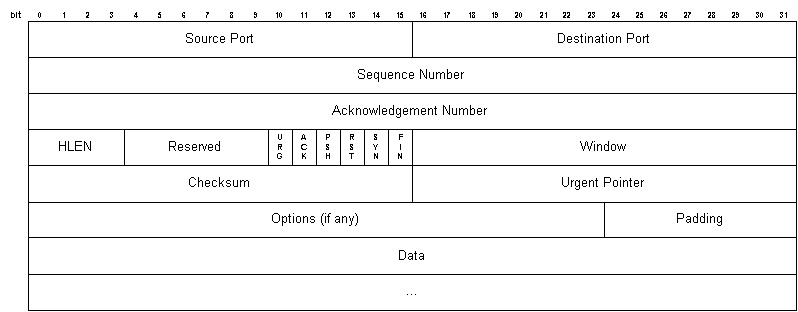
\includegraphics[width=0.75\textwidth]{images/tcp_frame.jpg}
    \end{figure}
\end{flushleft}